\section{ARC's Approach}
\label{sec:approach}

%ARC aims to automatically repair concurrency bugs like the one presented in
%Sect.~\ref{sec:motivation}.

% A high-level overview of ARC's approach is presented in Fig.~\ref{fig:process}.

There are two inputs to ARC: A ``buggy'' concurrent Java program and a JUnit test
suite. The test suite is necessary as it acts as an oracle to determine if bugs still exists in the program. One limitation of ARC (and of other
related automatic bug fixing techniques mentioned in
Sect.~\ref{sec:related_works}) is that it can only fix bugs detectable by the
test suite.

% \begin{figure}[h]
%   \centering
%   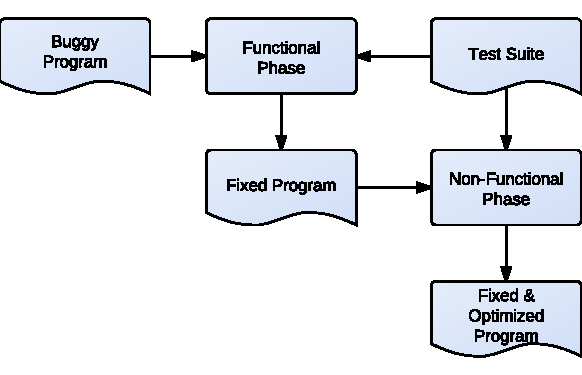
\includegraphics[width=7.0cm]{figures/process.pdf}
%   \caption{High Level Overview of ARC's Repair and Optimization Process}
%   \label{fig:process}
% \end{figure}

%ARC's complete approach is accomplished in two phases, the \textit{Functional
%Phase} and the \textit{Non-Functional Phase}. Both are similar in terms of the
%steps they follow, with slight variations to accomplish different goals. The
%first phase attempts to fix the buggy program while the second attempts to
%optimize its performance.

The following sections detail the fixing process as shown in
Fig.~\ref{fig:phases_internals}. We describe each step in the process in the order they occur. The key aspect of ARC's approach occur in the mutation and evaluation steps.

\begin{figure}[t!]
  \centering
  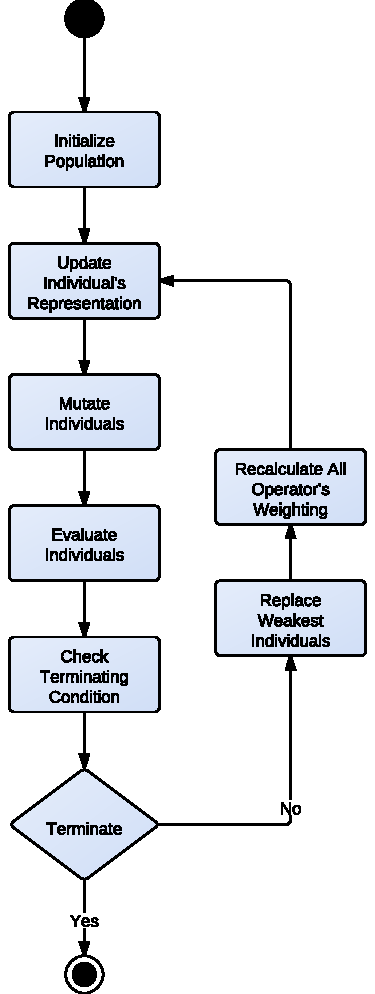
\includegraphics[width=7cm]{figures/phases.pdf}
  \caption{Detailed view of ARC's approach to concurrency bug repair}
  \label{fig:phases_internals}
\end{figure}

\subsection{Update Population}
\label{sec:update_population}

In the first step in the ARC approach the population of individuals is updated. For each
individual the previous generation (or the original program if ARC is just
starting) is copied to the current generation. Each individual contains their
own version of the program and the different versions evolve independently of each other.

% For the non-functional phase ARC has already produced the fixed
% program so each individual receives a copy of the fixed program to optimize.

\subsection{Update Individual's Representation}
\label{sec:update_individual_representation}

At this step ARC updates the individual's representation, which is accomplished
by generating the possible mutations from the current generation's program (which
is copied from the previous generation).

%Internally ARC keeps track of the mutants using a
%representational form as shown in Table~\ref{tbl:individual_representation}. As
%there exists multiple types of mutations, individuals are represented using a
%2-dimensional array of the mutation operators and the number of mutation
%instances generated.

%\begin{table}[h]
%\begin{center}
%\caption{An example representation of an individual, each 0 represents an
%instance of that mutation type that has been generated. It is possible for up
%to $n$ mutation operators with no-limit to the number of instances per
%operator.}
%\begin{tabular}{|l|l|}
%\hline
%\textbf{Operator} & \textbf{Instances}\\
%\hline
%Mutation 1 & 0\\
%\hline
%Mutation 2 & 0 0 0\\
%\hline
%Mutation 3 & --\\
%\hline
%\ldots & \ldots\\
%\hline
%Mutation $n$ & 0 0\\
%\hline
%\end{tabular}
%\label{tbl:individual_representation}
%\end{center}
%\end{table}

\begin{table}[t!]
\caption{Set of mutation operators used by ARC.}
\begin{center}
\begin{tabular}{|l|l|c|c|}
\hline
\textbf{Operator Description} & \textbf{Acronym} \\
\hline
Add synchronized around synchronized & ASAS \\
\hline
Add synchronized around variable & ASAV \\
\hline
Add synchronized in method header & ASIM \\
\hline
Add synchronized around method & ASM  \\
\hline
Change synchronized order & CSO  \\
\hline
Expand synchronized before & EXSB  \\
\hline
Expand synchronized after & EXSA  \\
\hline
Remove synchronized around synchronized & RSAS  \\
\hline
Remove synchronized around variable & RSAV  \\
\hline
Remove synchronized in method header & RSIM  \\
\hline
Remove synchronized around method & RSM  \\
\hline
\end{tabular}
\label{tbl:operators}
\end{center}
\end{table}

\begin{figure}[t!]
\vspace{2mm}
\begin{minipage}{5cm}

\footnotesize{\textbf{ Program $P$:}}
\begin{lstlisting}[language=Java, morekeywords={synchronize}]
obj.write(var1);
synchronized(lock){
  myHash.remove(var1);
}
\end{lstlisting}
\end{minipage}\hfill
\begin{minipage}{5cm}
\footnotesize{\textbf{ Program $P'$:}}
\begin{lstlisting}[language=Java, morekeywords={synchronize}]
synchronized(lock){
  obj.write(var1);
  myHash.remove(var1);
}
\end{lstlisting}
\end{minipage}

\caption{An example of the EXSB (expand synchronization before) mutation
operator.}
\label{fig:EXSB_example}
\end{figure}

The set of mutation operators ARC uses are listed in Table~\ref{tbl:operators},
and have mostly been derived by reversing the ConMAn operators~\cite{BCD06}. The ConMAn operators are used in mutation testing to create bugs while the ARC operators are used to fix bugs. The ARC operators are implement in 
TXL~\cite{CHP91} using pattern matching and replacement rules. An example of one of the ARC operators, 
EXSB, is shown in Fig.~\ref{fig:EXSB_example}. Each mutant
that is generated from the program creates a new mutant instance for that
individual of the mutation type.

% Original table with functional and non-functional
%\begin{table}[h]
%\caption{Set of mutation operators used by ARC. Each mutation operator is
%active during the indicated phases.}
%\begin{center}
%\begin{tabular}{|l|l|c|c|}
%\hline
%\textbf{Operator} & \textbf{Acronym} & \textbf{Functional} & \textbf{Non-Functional}\\
%\hline
%Add synch. around synch. & ASAS & $\surd$ &\\
%\hline
%Add synch. around variable & ASAV & $\surd$ &\\
%\hline
%Add synch. in method header & ASIM & $\surd$ &\\
%\hline
%Add synch. around method & ASM & $\surd$ &\\
%\hline
%Change synch. order & CSO & $\surd$ &\\
%\hline
%Expand synch. before & EXSB & $\surd$ &\\
%\hline
%Expand synch. after & EXSA & $\surd$ &\\
%\hline
%Remove synch. around synch. & RSAS & $\surd$ & $\surd$\\
%\hline
%Remove synch. around variable & RSAV & $\surd$ & $\surd$\\
%\hline
%Remove synch. in method header & RSIM & $\surd$ & $\surd$\\
%\hline
%Remove synch. around method & RSM & $\surd$ & $\surd$\\
%\hline
%Shrink synch. before & SHSB & & $\surd$\\
%\hline
%Shrink synch. after & SHSA & & $\surd$\\
%\hline
%\end{tabular}
%\label{tbl:operators}
%\end{center}
%\end{table}

% Modified table of functional only operators


As ARC mutates synchronization aspects of programs, the mutations themselves
can alter the occurrence of future mutations. This causing the search space of
possible mutations to potentially changes in every generation.

% Thus ARC must update the representation according to the latest state of the
% program's source code each generation.

\subsection{Apply a Mutation to an Individual}
\label{sec:mutate_individuals}

Once all mutants are generated for each individual, ARC selects a type of
mutation (e.g. EXSB) and then an instance of it (e.g. 4$^{th}$ mutant
generated) from those available. The selected mutation is applied and becomes
the current generation's code. ARC at this point will re-compile the project to
ensure that the mutation consists of valid syntax. In the situation that the
compilation fails another mutation type and instance is selected until a valid
combination is found.

ARC can leverage historical information about previous evaluations of the
mutation operators along with information about the current dominating bug type
found during testing. We use a weighted heuristic to select the mutation operator. Specifically, previous mutation operator evaluations and dominating bug types add weight to operators that
have been successful in the past, as well as to select operators that appear to
reduce the occurrences of either deadlocks or data races more often. This
heuristic is further detailed in
Sect.~\ref{sec:recalculate_operator_weighting}. Currently, mutation operator selection
is weighted but the mutant instances are selected randomly with equal
probability.

\subsection{Evaluate Individuals}
\label{sec:evalute_individuals}

A mutation may be beneficial, destructive or benign. We must evaluate it to
determine it's effect on the program. A key problem in evaluating mutants is the unpredictability of
thread interleavings. If a concurrency bug appears in only a few possible interleavings, how can we gain
confidence that a proposed fix actually works? 

ARC uses IBM's ConTest tool~\cite{EFN+02} to instrument the software under repair by injecting noise into the
program. The injected noise causes threads to randomly delay at different times during execution,
effectively causing each execution of the program to explore a different interleaving. By running the instrumented version of the program multiple times we gain more confidence that a larger set of the interleavings
are explored. Running the instrumented program multiple times is the most time
consuming aspect of ARC.

The number of successful ConTest executions are used to determine fitness:

\begin{footnotesize}
\begin{center}
$functional\ fitness(P) = (s \times sw) + (t \times tw)$
\end{center}
\end{footnotesize}
\begin{scriptsize}
\begin{center}
$s = \#\ of\ successful\ executions$ \\
$sw = success\ weighting$ \\
$t = \#\ of\ timeout\ executions$ \\
$tw = timeout\ weighting$
\end{center}
\end{scriptsize}

\noindent In determining fitness we consider both a successful execution and a timeout as positive factors. Timeouts are consider positive because given more time an execution that times out may result in a successful execution. We weight timeouts less than a successful execution as it could still result in a bug.

If ARC finds an individual that achieves 100\% successful executions, we need
to ensure it is truly a fix. It is possible that a proposed solution could
still contain a concurrency bug that escaped detection because the interleaving that exhibits the bug was not encountered by ConTest. To increase our confidence that a fix is correct we run ConTest
an additional number of times if all of the tests passed for the previous executions. The number of additional ConTest executions is usually some multiple of the previous number of runs. If the fix still holds even after this additional testing we feel confident the solution is indeed a true solution. If any of the additional executions fail,
the proposed fix is rejected and the evolutionary process continues.

\subsection{Check Terminating Condition}
\label{sec:check_terminating_condition}

ARC continues to evolve and evaluate individuals until
%some terminating condition is met. The following conditions are for the functional phase:
a solution is found or the
generational limit is reached. If a solution is found ARC outputs the modified program for the user to examine.
%The following conditions are for the non-
%functional phase: The population has converged (no improvement has been seen in
%$x$ generations), no more mutations are generated, or the generational limit is
%hit.

\subsection{Replace Weakest Individuals}
\label{sec:replace_weakest_individuals}

With any evolutionary algorithm it is entirely possible for an individual to
stray down a path leading to little or no improvement. To encourage individuals
to explore more fruitful areas of the state space we employ a replacement
strategy that replaces the lower $w$ percentage of individuals with a random
individual from the upper $x$ percent or the original buggy program with $y$
percent chance. These replacements only occur after an individual has
underperformed for $z$ generations. We believe the \textit{competent programmer
hypothesis}~\cite{ABD+79} applies so the corrected program isn't very far away
in the search space from the original buggy program.
%Therefore we provide a chance for an under-performing individual to reset
%back the initial state to allow the individual to explore from the starting
%point again.

\subsection{Recalculate All Operator's Weighting}
\label{sec:recalculate_operator_weighting}

As mentioned in Sect.~\ref{sec:mutate_individuals} ARC utilizes a heuristic
approach in selecting the mutation operator. A sliding window of $n$
generations is used to determine the success of previously applied mutation
operators. Operators that improve fitness are weighted more heavily and are
more likely to be selected. A sliding window is used to prevent dominance of
operators and to allow for flexibility in changing the weightings based on
recent history. The weighting is designed to ensure the chance of selecting an
operator is always greater than zero regardless of their performance.
%To ensure this approach is up to date the current weighting for
%each operator is recalculated based on the new feedback received from the
%population.
We consider a separate weighting for data races and deadlocks to remain
accurate in the use of this heuristic based on the current bug ARC is trying to
fix.
